\documentclass[a4paper]{article}

\usepackage{INTERSPEECH2015}

\usepackage{graphicx}
\usepackage{amssymb,amsmath,bm}
\usepackage{textcomp}

\def\vec#1{\ensuremath{\bm{{#1}}}}
\def\mat#1{\vec{#1}}

\usepackage{cleveref}
\usepackage{caption}

\usepackage[dvipsnames]{xcolor}
\newcommand{\TODO}[1]{{\color{red}\textbf{[TODO #1]}}}

\sloppy % better line breaks
\ninept

\title{A CAPT tool for training and research on lexical stress errors in German}

%%%%%%%%%%%%%%%%%%%%%%%%%%%%%%%%%%%%%%%%%%%%%%%%%%%%%%%%%%%%%%%%%%%%%%%%%%
%% If multiple authors, uncomment and edit the lines shown below.       %%
%% Note that each line must be emphasized {\em } by itself.             %%
%% (by Stephen Martucci, author of spconf.sty).                         %%
%%%%%%%%%%%%%%%%%%%%%%%%%%%%%%%%%%%%%%%%%%%%%%%%%%%%%%%%%%%%%%%%%%%%%%%%%%
%\makeatletter
%\def\name#1{\gdef\@name{#1\\}}
%\makeatother
%\name{{\em Firstname1 Lastname1, Firstname2 Lastname2, Firstname3 Lastname3,}\\
%      {\em Firstname4 Lastname4, Firstname5 Lastname5, Firstname6 Lastname6,
%      Firstname7 Lastname7}}
%%%%%%%%%%%%%%% End of required multiple authors changes %%%%%%%%%%%%%%%%%

\makeatletter
\def\name#1{\gdef\@name{#1\\}}
\makeatother \name{{\em%
  Anjana Sofia Vakil
  %Author Name$^1$, Co-author Name$^2$
  }}

\address{%
  %$^1$Author Affiliation \\
  %$^2$Co-author Affiliation \\
  Department of Computational Linguistics \& Phonetics\\
  Saarland University, Saarbr\"{u}cken, Germany\\
  {\small \tt 
  anjanav@coli.uni-saarland.de}
}
%\twoauthors{Karen Sp\"{a}rck Jones.}{Department of Speech and Hearing \\
%  Brittania University, Ambridge, Voiceland \\
%  {\small \tt Karen@sh.brittania.edu} }
%  {Rose Tyler}{Department of Linguistics \\
%  University of Speechcity, Speechland \\
%  {\small \tt RTyler@ling.speech.edu} }

%
\begin{document}

  \maketitle
  %
  \begin{abstract}
    This demonstration presents a prototype tool for Computer-Assisted Pronunciation Training (CAPT) in German.  
  \end{abstract}
  \noindent{\bf Index Terms}: speech recognition, human-computer interaction, computational paralinguistics


%	\section{System overview}
%	\label{sec:overview}
	
	This demonstration presents \textbf{de-stress}\footnote{\texttt{github.com/vakila/de-stress}}: the German (\textbf{de}) \textbf{S}ystem for \textbf{T}raining and \textbf{R}esearch on \textbf{E}rrors in \textbf{S}econd-language \textbf{S}tress. 
%
%Implemented as a web application 
%%in the Java-based language Groovy\footnote{\texttt{groovy-lang.org}} using the Grails web framework,\footnote{\texttt{grails.org}} 
%de-stress and its source code are openly available online.\footnote{\texttt{github.com/vakila/de-stress}}

%\Cref{fig:hourglass-ITS} provides a conceptual overview of the tool, which 
This prototype CAPT tool provides a variety of options for diagnosis of and feedback on lexical stress errors, and could potentially be a useful component of an intelligent CAPT system. 



 Via a simple web interface, the system presents a student with a German sentence,
 %(taken from the IFCASL corpus), 
 with one of the words highlighted as the target word for that exercise. The student is prompted to submit an utterance of that sentence for assessment and feedback, with the instruction to focus on the accurate expression of the lexical stress pattern of the target word. The student's utterance is subsequently analyzed for lexical stress errors using a variety of diagnostic approaches (see \cref{chap:diagnosis}), and finally the student is presented with one or more types of feedback on their realization of lexical stress in the analyzed utterance (see \cref{chap:feedback}). \Cref{fig:interface:student} presents a screenshot of the interface presenting such feedback.

	\begin{figure}[htb]
		\centering
		%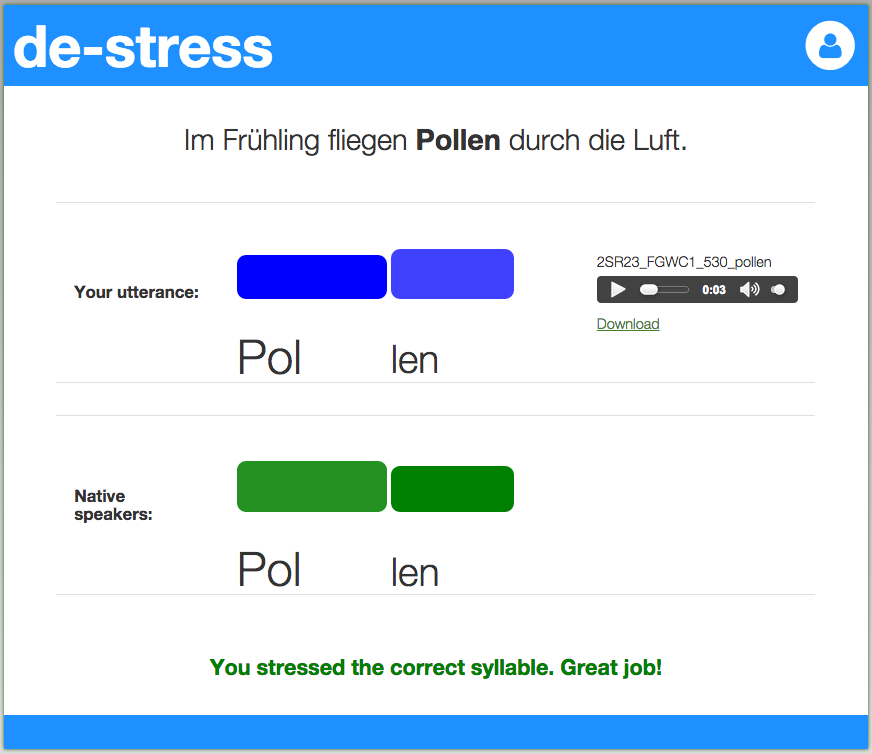
\includegraphics[width=\columnwidth]{../../img/screenshots/StudentInterface-userIcon}
		%\caption{The student-facing interface of de-stress}
		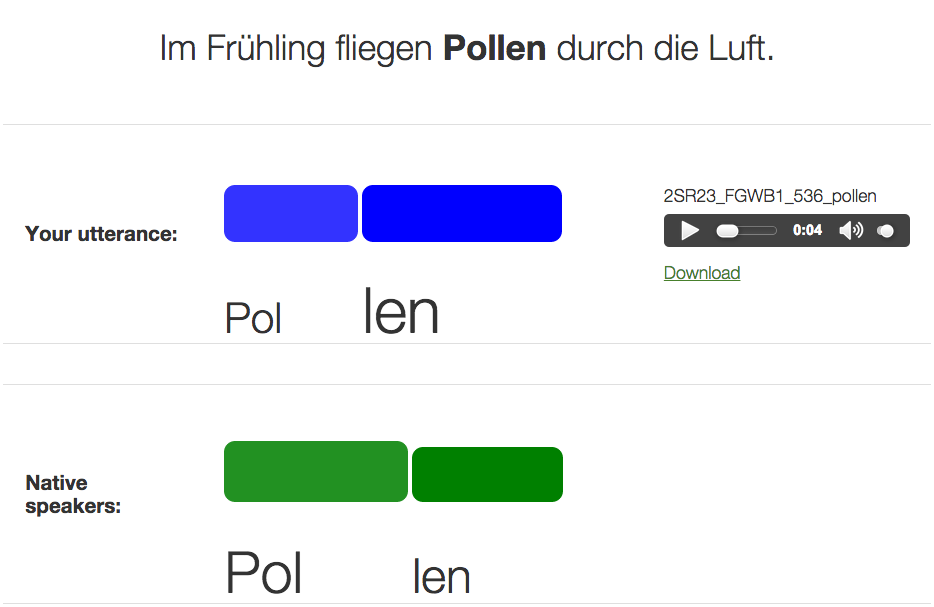
\includegraphics[width=\columnwidth]{../../img/screenshots/graphicalFB-weka-plusTextStyle}
		\caption{Example of feedback delivery in de-stress}
		\label{fig:interface:student}
	\end{figure}

In addition to this student-facing interface, 
%the tool also implements an interface through which 
an administrative interface allows
a language teacher or a researcher of L2 language acquisition 
%can 
to
create new exercises for students to complete, where each exercise features a specific combination of the various diagnostic methods and feedback types available in the system. By allowing fine-grained control over these features, de-stress enables researchers to create CAPT exercises with different features for the purposes of in vivo studies of the effectiveness of different feedback types, and allows teachers to create exercises matching the needs of their students. 
%The 
%%teacher- or researcher-facing
%administrative interface for exercise creation can be seen in \cref{fig:interface:teacher}.

%	\begin{figure}[htbp]
%		\centering
%		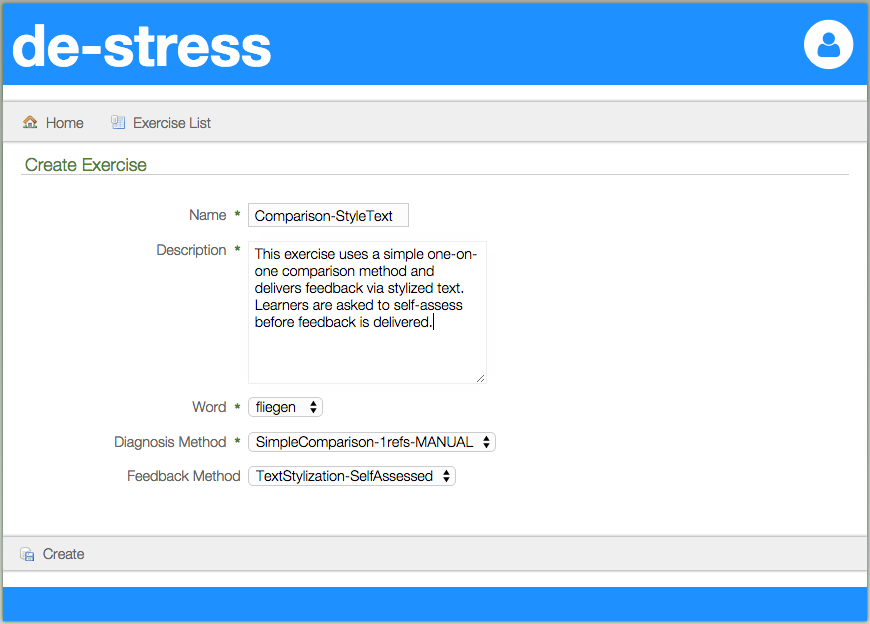
\includegraphics[width=\columnwidth]{../../img/screenshots/TeacherInterface-userIcon}
%		\caption{The interface of de-stress for teachers/researchers}
%		\label{fig:interface:teacher}
%	\end{figure}

%\TODO{This prototype tool} has thus been developed with both instructional and research applications in mind.
Both instructional and research applications have thus motivated the development of de-stress.
Unlike with some existing tools for diagnosis and feedback on pronunciation errors, learners can interact with the tool and interpret its feedback independently, i.e. without the assistance of a human instructor at their side.
At the same time, researchers can use this modular system to study the impact of various assessment and feedback types on learner outcomes, user engagement, and other factors impacting the success of a CAPT system. 
%
Once more is known about which diagnosis/feedback types should be delivered to which learners in which situations, this tool could become a useful component of a fully-fledged intelligent CAPT system, in which 
%learner models and other intelligent components
models of relevant aspects of the learning context (e.g. the student's skill level, progress, or personal preferences; the current learning objective or position in a sequence of exercises; etc.)
are used to automatically decide which modules of the tool to activate, as \cref{fig:hourglass-ITS} illustrates.

	\begin{figure}[tb] 
		\centering
		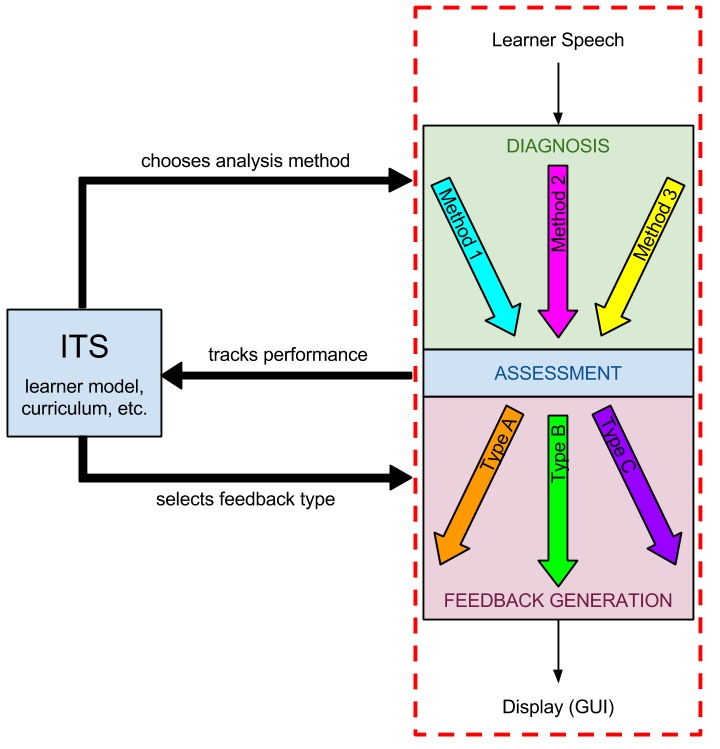
\includegraphics[height=.25\textheight]{../../img/hourglass-ITS} 
		\caption[Conceptual diagram of the prototype lexical stress CAPT tool]{Conceptual diagram of the prototype lexical stress CAPT tool (demarcated by dashed line) and its possible function in the context of a more comprehensive Intelligent Tutoring System (ITS).}
		\label{fig:hourglass-ITS}
	\end{figure}
	
%	\section{Error diagnosis options}
%	\label{sec:diag}
%	
%	\TODO{}
%	
%	\section{Feedback options}
%	\label{sec:fb}
%	
	\TODO{}
	
	


  %\newpage
  \eightpt
  \bibliographystyle{IEEEtran}

  \bibliography{mybib}

%  \begin{thebibliography}{9}
%    \bibitem[1]{Davis80-COP}
%      S.\ B.\ Davis and P.\ Mermelstein,
%      ``Comparison of parametric representation for monosyllabic word recognition in continuously spoken sentences,''
%      \textit{IEEE Transactions on Acoustics, Speech and Signal Processing}, vol.~28, no.~4, pp.~357--366, 1980.
%    \bibitem[2]{Rabiner89-ATO}
%      L.\ R.\ Rabiner,
%      ``A tutorial on hidden Markov models and selected applications in speech recognition,''
%      \textit{Proceedings of the IEEE}, vol.~77, no.~2, pp.~257-286, 1989.
%    \bibitem[3]{Hastie09-TEO}
%      T.\ Hastie, R.\ Tibshirani, and J.\ Friedman,
%      \textit{The Elements of Statistical Learning -- Data Mining, Inference, and Prediction}.
%      New York: Springer, 2009.
%    \bibitem[4]{YourName15-XXX}
%      F.\ Lastname1, F.\ Lastname2, and F.\ Lastname3,
%      ``Title of your INTERSPEECH 2015 publication,''
%      in \textit{Interspeech 2015 -- 16\textsuperscript{th} Annual Conference of the International Speech Communication Association, September 06--10, Dresden, Germany, Proceedings}, 2015, pp.~100--104.
%  \end{thebibliography}

\end{document}
